%   % !TEX root = ../../VIII,3_Rahmen-TeX_9-0.tex
%  
%   Band VIII, 3 N.~?? 	[XXX??.?]			Gerader Stoß 
%   Signatur/Tex-Datei:	LH_37_05_152r
%   RK-Nr. 	60344-1
%   Überschrift: 	(keine)
%   Titel: 			De motu centri potentiae???
%   Datierung:		???? bis ???? (a. St.?), eigh. (?)				??
%   Textfolge: 			vllt abbrechend / Fortsetzung in RK ??	??
%   WZ: 	Nr. 803004
%   edlabels:			7
%   Diagramme: 		1 (mit Entwurf) auf 152r + ganz unten noch ein Entwurf?
%   Dateien (PDF):
%   		LH_37_05_152_d1_152r
%
%   Erstaufnahme:			(wer?)
%   Bearbeitung MS ab: 		Juni 2020
%
%   NB: 			vielleicht abbrechend?
%
%
%
\selectlanguage{ngerman}
\frenchspacing
%
\begin{ledgroupsized}[r]{120mm}
\footnotesize
\pstart
\noindent\textbf{Überlieferung:}
\pend
\end{ledgroupsized}
%
\begin{ledgroupsized}[r]{114mm}
\footnotesize
\pstart \parindent -6mm
\makebox[6mm][l]{\textit{L}}%
Konzept:
LH~XXXVII~5~Bl.~152. 
Ein Blatt~2\textsuperscript{o},
nachträglich in 4\textsuperscript{o} gebrochen;
Wasserzeichen in der Blattmitte;
Papiererhaltungsmaßnahmen.
Zweidrittel Seiten auf Bl.~152~r\textsuperscript{o}, quer einspaltig beschrieben;
Bl.~152~v\textsuperscript{o} überliefert N.~\ref{RK60344_2}.
\pend
\end{ledgroupsized}
%
\vspace{5mm}
\begin{ledgroup}
\footnotesize
\pstart
\noindent%
\textbf{Datierungsgründe:}
Im Konzept N.~\ref{RK60344_1}, wie bereits in N.~\ref{RK57273},
%
ist Leibniz um eine Einführung des Begriffs des \textit{centrum potentiae} zweier Körper bemüht.
%
Nach der Definition erörtert Leibniz in N.~\ref{RK60344_1} die Eigenschaften der Bewegung des \textit{centrum potentiae}
%
und bestimmt, von den möglichen Bewegungen der zwei Körper ausgehend,
%
seine Lage vor und nach dem Stoß.
%
Dabei nimmt er auf S.~\refpassage{37_05_152r_7a}{37_05_152r_7b} 
%
ausdrücklich auf einen früheren Text Bezug, worin er die Lage des \textit{centrum} vor dem Stoß
%
bereits untersucht haben soll. Es handelt sich höchstwahrscheinlich um eine Anspielung auf N.~\ref{RK57273},
%
ein Konzept, das ebenfalls die Merkmale einer Einführung aufweist, 
%
aber tatsächlich nur die Konfiguration der Körper vor dem Stoß behandelt.
%
Somit muss N.~\ref{RK57273} (Mai bis Mitte Juni 1677) vor N.~\ref{RK60344_1} abgefasst worden sein.
\pend
%
%%%
%%%
\pstart
Zur weiteren Einkreisung der Entstehung von N.~\ref{RK60344_1} kann das Konzept N.~\ref{RK57274} herangezogen werden.
%
Dieses zählt neben N.~\ref{RK57277} und N.~\ref{RK57275} zu den Stücken im Zeitraum 1677 bis Januar 1678, die 
sich auf den Begriff und die Eigenschaften des \textit{centrum potentiae} berufen.
%
Als Terminus ante quem für N.~\ref{RK57274} kann  Mitte Juni 1677 ermittelt werden (siehe die Datierungsgründe). 
%
Unter der Annahme, dass die grundlegenden Ausführungen von N.~\ref{RK60344_1} 
%
(und N.~\ref{RK57273}) der Abfassung von N.~\ref{RK57274} vorausgingen, 
%
kann der genannte Ter- \makebox[1.0\textwidth][s]{minus ante quem übernommen werden,
%
woraus sich für N.~\ref{RK60344_1} die vorgeschlagene Datierungsspanne ergibt.}
\pend
\end{ledgroup}
%
%
\selectlanguage{latin}
\frenchspacing
% \newpage%
\vspace{7mm}
\pstart%
\normalsize%
\noindent%
\lbrack152~r\textsuperscript{o}\rbrack\
\pend
%
\count\Bfootins=1000%
\count\Afootins=1000%
\count\Cfootins=1000
%
\vspace{0.7em} %%%%%%%%% Diagramm 1
\centerline{%
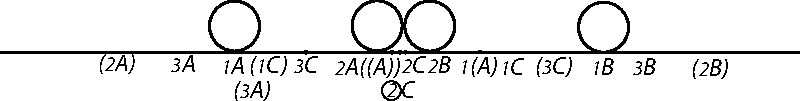
\includegraphics[width=0.9\textwidth]{%
gesamttex/edit_VIII,3/images/LH_37_05_152r_d.pdf%
}} 
\vspace{0.5em}
\centerline{%
\lbrack\textit{Fig.~1}\rbrack%
}
% \newpage%
\vspace{1.1em}
%
\pstart\noindent%
%
\edtext{}{%
\lemma{\hspace*{1,6mm}%
\lbrack\textit{Fig.~1}\rbrack%
}\killnumber%
\Cfootnote{%
In der Figur verwendet Leibniz zumeist Bezeichnungen der Form (\textit{{\scriptsize1}}\textit{A}) und ((\textit{{\scriptsize1}}\textit{A})), im Text dagegen \textit{{\scriptsize1}}(\textit{A}) und \textit{{\scriptsize1}}((\textit{A})). Ein gestrichener Entwurf zum Diagramm wird nicht wiedergegeben.%
}}%
%
%
\textit{{\scriptsize1}A} vel \textit{{\scriptsize1}}(\textit{A}) vel \textit{{\scriptsize1}}((\textit{A})) situs corporis \textit{A} primus, \textit{{\scriptsize2}A} %
\edtext{vel \textit{{\scriptsize2}}(\textit{A})}{\lemma{}\Bfootnote{vel \textit{{\scriptsize2}}(\textit{A}) \textit{erg.~L}}} %
%
situs secundus, seu ad quem\pend
%
\pstart\noindent
\edtext{\lbrack\textit{{\scriptsize1}B}\rbrack}{\lemma{}\Bfootnote{\textit{{\scriptsize1}A} \textit{ändert~Hrsg.} \textbar\ vel \textit{{\scriptsize2}B} \textit{gestr.} \textbar\ \dots~\textit{L}}} %
%
\newlength{\situsprimus}\settowidth{\situsprimus}{v \textit{{\scriptsize1}}(\textit{A}) vel \textit{{\scriptsize1}}((\textit{A})) situs corporis \textit{A} primus,}
\parbox[b][][b]{\situsprimus}{$\dotfill$}
\textit{{\scriptsize2}B} %
\edtext{vel \textit{{\scriptsize2}}(\textit{B})}{\lemma{}\Bfootnote{vel \textit{{\scriptsize2}}(\textit{B}) \textit{erg.~L}}}
\newlength{\situssecundus}\settowidth{\situssecundus}{situs secundus, seu ad quem}
\parbox[b][][b]{\situssecundus}{$\dotfill$}
\pend
%
\pstart\noindent
per motum pervenit.
\pend
\pstart\noindent%
\newlength{\permotum}\settowidth{\permotum}{per motum pervenit}%
\parbox[b][][b]{\permotum}{$\dotfill$}
\pend
\newpage
\count\Bfootins=1100%
\count\Afootins=1100%
\count\Cfootins=1100
\pstart
\textit{{\scriptsize1}C} est centrum potentiae\protect\index{Sachverzeichnis}{centrum potentiae} inter corpora \textit{{\scriptsize1}A} et \textit{{\scriptsize1}B} et recta \textit{{\scriptsize1}B}\textit{{\scriptsize1}C} est ad rectam \textit{{\scriptsize1}A}\textit{{\scriptsize1}C}, %
\edtext{ut factum ex}{\lemma{ut}\Bfootnote{\textit{(1)}~corpus \textit{A} ductum \textit{(2)}~factum~\textit{L}}} %
%
 corpore \textit{A} ducto in suam celeritatem,\protect\index{Sachverzeichnis}{factum ex corpore ducto in celeritatem} seu in viam, nempe rectam  %
\edtext{\textit{{\scriptsize1}A}\textit{{\scriptsize2}A}, ad factum}{\lemma{ad}\Bfootnote{\textit{(1)}~corpus \textit{(2)}~factum~\textit{L}}} %
%
ex corpore \textit{B} in suam %
\edtext{\lbrack celeritatem\rbrack,\protect\index{Sachverzeichnis}{factum ex corpore ducto in celeritatem}}%
{\lemma{}\Bfootnote{celeritatem \textit{erg.~Hrsg.}}} seu in %
\edtext{rectam \textit{{\scriptsize1}B}\textit{{\scriptsize2}B}. \textit{{\scriptsize2}C}}{\lemma{rectam}\Bfootnote{\textit{(1)}~\textit{{\scriptsize1}A} \textit{(2)}~\textit{{\scriptsize1}B}\textit{{\scriptsize2}B}. \textit{(a)}~({\scriptsize \textit{2}}) est \textit{(b)}~\textit{{\scriptsize2}}(\textit{C}) est secundus \textit{(c)}~\textit{{\scriptsize2}C}~\textit{L}}} %
%
est secundus centri potentiae locus, cum corpora venere in \textit{{\scriptsize2}A} et \textit{{\scriptsize2}B}. 
\pend
%
\pstart 
Centrum potentiae semper inter duo corpora  %
\edtext{situm est. Ergo}{\lemma{situm est}\Bfootnote{\textit{(1)}~, seu \textit{(2)}~. Ergo~\textit{L}}} %
%
 si  %
\edtext{\textit{{\scriptsize1}A} est dexterius (sinisterius) quam \textit{{\scriptsize1}C} erit etiam dexterius (sinisterius) quam}{\lemma{\textit{{\scriptsize1}A} est}\Bfootnote{\textit{(1)}~sinisterius \textit{(2)}~dexterius \textbar\ (sinisterius) \textit{erg.}\ \textbar\ %
quam \textit{{\scriptsize1}C} erit etiam dexterius \textbar\ (sinisterius) \textit{erg.}\ \textbar\ quam~\textit{L}}} %
%
\textit{{\scriptsize1}B}. %
\edtext{Item si}{\lemma{}\Bfootnote{Item \textbar\ item \textit{gestr.} \textbar\ si~\textit{L}}} %
%
\textit{{\scriptsize1}A} est dexterius (sinisterius) quam \textit{{\scriptsize1}B} erit etiam dexterius (sinisterius) quam \textit{{\scriptsize1}C}.%
\pend
%
\pstart
Ad calculum peragendum comperi necesse esse, ut %
\edtext{investig\lbrack et\rbrack ur}{\lemma{}\Bfootnote{investigentur \textit{L ändert~Hrsg.}}} in omnibus casibus situs quem habent inter se %
\,\edtext{\textso{1\textsuperscript{\textso{\,mo}}}\, puncta}{\lemma{\textso{1\textsuperscript{\,mo}}}\Bfootnote{\textit{(1)}~duo \textit{(2)}~puncta~\textit{L}}} %
%
tria: \begin{tabular}[t]{c}\textit{{\scriptsize1}B}.\textit{{\scriptsize2}B}.\textit{{\scriptsize2}C}.\\{\scriptsize \textit{1}}\textit{A}.\textit{{\scriptsize2}A}.\textit{{\scriptsize2}C}\end{tabular}
%
\,\textso{2\textsuperscript{\textso{\,do}}}\, puncta tria: \begin{tabular}[t]{c}\textit{{\scriptsize1}B}.\textit{{\scriptsize1}C}.\textit{{\scriptsize2}C}.\\{\scriptsize \textit{1}}\textit{A}.\textit{{\scriptsize1}C}.\textit{{\scriptsize2}C}\end{tabular} %
\pend
%
\pstart
Ponamus \textit{{\scriptsize1}B} dexterius quam \textit{{\scriptsize1}A}, erit et \textit{{\scriptsize1}B} dexterius quam \textit{{\scriptsize1}C}, et \textit{{\scriptsize1}A} sinisterius quam \textit{{\scriptsize1}C}. %
\pend
%
\pstart
Item erit et \textit{{\scriptsize2}B} dexterius quam \textit{{\scriptsize2}A} et rursus \textit{{\scriptsize2}B}
%
\newlength{\dexterius}\settowidth{\dexterius}{dexterius q}
\parbox[b][][b]{\dexterius}{$\dotfill$}
\textit{{\scriptsize2}C} et \textit{{\scriptsize2}A} sinisterius 
%
\edlabel{37_05_152r_1a}%
\edtext{}{{\xxref{37_05_152r_1a}{37_05_152r_1b}}%
\lemma{quam \textit{{\scriptsize2}C}.}%
\Bfootnote{\textit{(1)}~Videndum an \textit{(a)}~semper aliquod sumi possit \textit{(b)}~corpus motum, quod semper \textit{(2)}~\textso{Semper}~\textit{L}}}%
quam \textit{{\scriptsize2}C}.
\pend
%
\pstart
\textso{Semper}%
\edlabel{37_05_152r_1b}%
\textso{ intelligi potest centrum potentiae,}\protect\index{Sachverzeichnis}{centrum potentiae}%
\textso{ et aliquod ex corporibus}\lbrack,\rbrack\ \textso{tendere in eandem partem}. 
%
Sit illud corpus \textit{B}. Si corpora sibi occurrunt aut a se invicem divergunt, tunc centrum potentiae\protect\index{Sachverzeichnis}{centrum potentiae} aut quiescit aut movetur. Si quiescit, fingatur moveri sed motu tardissimo\protect\index{Sachverzeichnis}{motus tardissimus} et salvus erit calculus; sin movetur, tunc necessario in alterutram partem movetur. Ergo necessario movetur in partem in quam alterutrum corporum movetur, quoniam nullum %
\edtext{latus assignari}{\lemma{latus}\Bfootnote{\textit{(1)}~assignatur \textit{(2)}~assignari~\textit{L}}} %
%
potest, in %
\edtext{\lbrack quod\rbrack}{\lemma{}\Bfootnote{quem \textit{L ändert~Hrsg.}}} non in casu concursus\protect\index{Sachverzeichnis}{concursus} aut divergentiae\protect\index{Sachverzeichnis}{divergentia} aliquod corporum moveatur. Si vero %
\edtext{corpora ambo}{\lemma{corpora}\Bfootnote{\textit{(1)}~non ten \textit{(2)}~ambo~\textit{L}}} %
%
tendant in eandem partem, id est, neque divergant, neque occurrant, utique manifeste et centrum potentiae,\protect\index{Sachverzeichnis}{centrum potentiae} in eandem movetur %
\edtext{partem. Huc}{\lemma{partem.}\Bfootnote{\textit{(1)}~Ex hoc porro \textit{(2)}~Huc~\textit{L}}} %
%
pertinet, et si aliquod corporum quiescat, nam quietem\protect\index{Sachverzeichnis}{quies} habeo pro motu tardissimo.\protect\index{Sachverzeichnis}{motus tardissimus} %
\pend
%
\pstart
\textso{Semper intelligi potest aliquod corporum sequi centrum potentiae }\protect\index{Sachverzeichnis}{centrum potentiae}%
\edtext{\textso{excepto divergentiae casu},}{\lemma{}\Bfootnote{\textso{excepto divergentiae casu} \textit{erg.~L}}} %
%
id est non tantum in eandem ire partem, sed %
et ipso \makebox[1.0\textwidth][s]{esse posterius,
%
seu (si motus fingatur a dextro ad sinistrum) dexterius. Ostendo, nam si}
\pend
\newpage
\pstart \noindent%
\edtext{corpora sibi}{\lemma{corpora}\Bfootnote{\textit{(1)}~concurrant \textit{(2)}~sibi~\textit{L}}} %
%
occurrant, tunc id quod in eandem it partem cum centro potentiae\protect\index{Sachverzeichnis}{centrum potentiae} semper ipso est posterius. Nam centrum potentiae\protect\index{Sachverzeichnis}{centrum potentiae} propius est corpori opposito, seu sito versus latus in quod itur, ergo prius est, et corpus est %
\edtext{posterius. Si}{\lemma{posterius.}\Bfootnote{\textit{(1)}~Si corpora divergant tunc \textit{(2)}~Si~\textit{L}}} %
%
corpora in easdem partes inter se et cum centro potentiae\protect\index{Sachverzeichnis}{centrum potentiae} tendant, tunc alterutrum eorum erit centro potentiae\protect\index{Sachverzeichnis}{centrum potentiae} prius, alterutrum posterius, ergo semper %
\edtext{aliquod sequetur}{\lemma{aliquod}\Bfootnote{\textit{(1)}~centrum \textit{(2)}~sequetur~\textit{L}}} %
%
centrum potentiae.\protect\index{Sachverzeichnis}{centrum potentiae} 
%
Unus casus deest, cum divergunt, tunc enim corpus praecedit, potest tamen determinari casus ille aliunde sine calculo, quemadmodum in caeteris quoque omnibus. Id sciri potest sumendo casum divergentiae\protect\index{Sachverzeichnis}{divergentia} velut %
\edtext{inversum occursus,\protect\index{Sachverzeichnis}{occursus}}{\lemma{inversum}\Bfootnote{\textit{(1)}~concursus \textit{(2)}~occursus,~\textit{L}}} %
%
et posteriorem. Idemque in genere est, intelligendum de motu quo a se invicem 
%
\edlabel{37_05_152r_6a}%
\edtext{}{% NEUER ABSATZ UND VARIANTEN – "discedunt"
{\xxref%
{37_05_152r_6a}{37_05_152r_6b}}%
\lemma{discedunt}%
\Bfootnote{%
\textit{(1)}~: %
\textit{(2)}~. Alibi
\textit{L}%
}}%
discedunt.
\pend
%
\pstart 
%
\hspace{1mm}\hspace{-1mm}% Trick, weil \edlabel nicht zu \par-Beginn sein darf
%
\edlabel{37_05_152r_7a}%
\edtext{}{% C-Footnote
{\xxref%
{37_05_152r_7a}{37_05_152r_7b}}%
\lemma{Alibi \lbrack...\rbrack\ concursum}%
\Cfootnote{%
Siehe N.~\ref{RK57273}, S.~\refpassage{37_05_146-147_17a}{37_05_146-147_17b}.}}%
%
Alibi\edlabel{37_05_152r_6b}	% 
%
jam excussimus situm %
\edtext{horum punctorum a statu}{\lemma{horum}\Bfootnote{\textit{(1)}~signorum \textit{(2)}~punctorum \textit{(a)}~ante concursum \textit{(b)}~a statu~\textit{L}}} %
%
ante concursum\protect\index{Sachverzeichnis}{concursus} usque ad concursum.\edlabel{37_05_152r_7b}
%
Nunc %
\edtext{consideremus a concursu\protect\index{Sachverzeichnis}{concursus} ad statum}{\lemma{consideremus a}\Bfootnote{\textit{(1)}~statu concursus \textit{(2)}~concursu \textit{(a)}~a statu \textit{(b)}~ad statum~\textit{L}}} %
%
 post concursum. %
\edtext{Et primum consideremus}{\lemma{Et}\Bfootnote{\textit{(1)}~quia primum manifestum est  \textit{(2)}~primum consideremus~\textit{L}}} %
%
 situm punctorum 
%
\begin{tabular}[t]{c}\textit{{\scriptsize3}B}.\textit{{\scriptsize3}C}.\textit{{\scriptsize2}C},\\
\textit{{\scriptsize3}A}.\textit{{\scriptsize3}C}.\textit{{\scriptsize2}C}\end{tabular}
%
item situm punctorum 
%
\begin{tabular}[t]{c}\textit{{\scriptsize3}B}.\textit{{\scriptsize2}B}.\textit{{\scriptsize2}C}.\\
\textit{{\scriptsize3}A}.\textit{{\scriptsize2}A}.\textit{{\scriptsize2}C}\end{tabular} 
%
Ubi imaginando calculi causa divergentiam\protect\index{Sachverzeichnis}{divergentia} esse 
%
\edtext{concurs\lbrack u\rbrack m\protect\index{Sachverzeichnis}{concursus}}{%
\lemma{}%
\Bfootnote{%
concursuum %
\textit{L ändert~\mbox{Hrsg.}}%
}}
 et elongationem\protect\index{Sachverzeichnis}{elongatio} esse appropinquationem,\protect\index{Sachverzeichnis}{appropinquatio} tunc %
\edtext{videndum quodnam corpus}{\lemma{videndum}\Bfootnote{\textit{(1)}~an \textit{(2)}~quod corpus \textit{(3)}~quodnam corpus~\textit{L}}} %
%
 in eandem eat partem cum %
\edtext{centro potentiae,\protect\index{Sachverzeichnis}{centrum potentiae}}{\lemma{centro}\Bfootnote{\textit{(1)}~gravitatis, \textit{(2)}~potentiae,~\textit{L}}} %
%
ipsumque %
\edtext{sequatur. Manifestum}{\lemma{sequatur.}\Bfootnote{\textit{(1)}~Primum si duo corpora occurrerint, tunc divergent. Nam quia \textit{(2)}~Manifestum~\textit{L}}} %
%
autem illud corpus in cujus partem ivit %
\edtext{centrum potentiae\protect\index{Sachverzeichnis}{centrum potentiae}}{\lemma{centrum}\Bfootnote{\textit{(1)}~gravitatis \textit{(2)}~potentiae~\textit{L}}} %
\edtext{ex \textit{{\scriptsize2}C} in \textit{{\scriptsize3}C,}}{\lemma{ex}\Bfootnote{\textit{{\scriptsize2}C} in \textit{{\scriptsize3}C} \textit{erg.~L}}} %
%
pro illo sumi posse, quod ipsum sequi intellegeretur si rediret ex \textit{{\scriptsize3}C} in \textit{{\scriptsize2}C}. Illud tantum videndum an quod ante secutum est corpus nunc non sit illud quod sequatur. Idque %
\edtext{manifestum est, nam}{\lemma{manifestum est,}\Bfootnote{\textit{(1)}~quia illud corpus in cujus tendit partem seque \textit{(2)}~nam~\textit{L}%
}}
%
semper unumquodque
%
\edtext{corpus a qua}{%
\lemma{corpus}%
\Bfootnote{%
\textit{(1)}~ab %
\textit{(2)}~a qua%
~\textit{L}%
}}
%
est parte, in ea %
\edtext{}{{\xxref{KZeitz199}{KZeitz200}}%
{\lemma{manet}\Bfootnote{%
\textit{(1)}~, deinde \textit{(a)}~corp \textit{(b)}~corpus quod sequitur %
\textit{(2)}~inter \textit{{\scriptsize3}C} %
\textit{(3)}~. Ponendo %
\textit{(a)}~\textit{C} %
\textit{(b)}~\textit{{\scriptsize2}C} 
tendere sinistrorsum 
\textit{(aa)}~erit
\textit{(bb)}~et
\textit{(aaa)}~\textit{B}
\textit{(bbb)}~\textit{{\scriptsize2}B} \lbrack...\rbrack\ erit
\textit{(aaaa)}~\textit{A} sinisterius quam \textit{{\scriptsize3}C},
\textit{(bbbb)}~\textit{{\scriptsize2}A} sinisterius quam \textit{{\scriptsize2}C},
\textit{L}}}}%
\edlabel{KZeitz199}manet. Ponendo \textit{{\scriptsize2}C} tendere sinistrorsum et \textit{{\scriptsize2}B} quoque ipsum sinistrorsum sequi, erit  \textit{{\scriptsize2}A} sini- \makebox[1.0\textwidth][s]{sterius quam \textit{{\scriptsize2}C},\edlabel{KZeitz200}%
 %
%
imo et \textit{{\scriptsize3}A} sinisterius quam \textit{{\scriptsize3}C}.
%
Ergo fingendo redire \textit{{\scriptsize3}A} in \textit{{\scriptsize2}A}, et \textit{{\scriptsize3}C}}
\pend
\newpage
\pstart
\noindent  in \textit{{\scriptsize2}C} manifestum  est sequi \textit{A} ipsum \textit{C}. (\protect\vphantom)Ponendo scilicet motum ipsius \textit{A} et \textit{C} semper esse uniformem\protect\index{Sachverzeichnis}{motus uniformis} seu %
\edtext{nunquam nunc praeter\lbrack veh\rbrack ere nunc}{\lemma{nunquam}\Bfootnote{\textit{(1)}~praeterevhere \textit{\lbrack!\rbrack} \textit{(2)}~nunc \textbar\ praeterquere \textit{ändert~Hrsg.} \textbar\ nunc~\textit{L}}} %
%
rursus a tergo 
%
\edlabel{37_05_152r_2a}%
relinqui\protect\vphantom().%
\edtext{}{{\xxref{37_05_152r_2a}{37_05_152r_2b}}\lemma{relinqui).}\Bfootnote{\textit{(1)}~Illud co \textit{(2)}~Si~\textit{L}}} %
%
\pend
%
\pstart 
Si%
\edlabel{37_05_152r_2b} 
%
corpora sibi occurrerunt, quaeritur quis sit situs %
\edtext{corporis \textit{B}.}{\lemma{corporis}\Bfootnote{\textit{(1)}~\textit{A} \textit{(2)}~\textit{B}.~\textit{L}}} %
%
Nam ille nunc quaerendus, seu \textit{{\scriptsize3}B}.\textit{{\scriptsize3}C}.\textit{{\scriptsize2}C} et \textit{{\scriptsize3}B}.\textit{{\scriptsize2}B}.\textit{{\scriptsize2}C}. 
%
Ac primum si corpora sibi occurrerunt, necesse est unum eorum retrocessisse quia enim \textit{C} progressum est, hinc \textit{A} quod ab latere sinistro est, in quod tendit, necessario retrocessit, quaeritur
%
\edtext{\lbrack an\rbrack}{\lemma{}\Bfootnote{an \textit{erg.~Hrsg.}}} 
%
alterum 
%
\edtext{\textit{B}}{%
\lemma{}%
\Bfootnote{%
\textit{B} %
\textit{erg.~L}%
}}
%
retrocesserit, an sit progressum quia celeritatum differentiae\protect\index{Sachverzeichnis}{differentia celeritatum} sunt ut corpora %
\edtext{reciproce,}{\lemma{reciproce}\Bfootnote{\textit{erg.~L}}} %
%
ergo potentiarum quoque differentiae\protect\index{Sachverzeichnis}{differentia potentiarum} %
\rule[0cm]{0mm}{16pt}\edtext{sunt aequales,}{\lemma{sunt}\Bfootnote{\textit{(1)}~ut corpora \textbar\ reciproce \textit{erg.}\ \textbar\  \textit{(2)}~aequales,~\textit{L}}} %
%
seu
%
\edlabel{37_05_152r_3a}%
$\displaystyle\frac{a}{b}\sqcap \displaystyle\frac{m-f}{e-i}$. Ergo%
\edlabel{37_05_152r_3b}%
\edtext{}{{\xxref{37_05_152r_3a}{37_05_152r_3b}}\lemma{seu $\displaystyle\frac{a}{b}\sqcap \displaystyle\frac{m-f}{e-i}$}\Bfootnote{\textit{(1)}~, seu $\displaystyle\frac{a^2b}{ab^2}\sqcap \displaystyle\frac{mb-fb}{}$ \textit{(2)}~. Er \textit{(3)}~. Ergo~\textit{L}}} %
%
$\displaystyle\frac{a}{b}\smallfrown \displaystyle\frac{b}{a}\sqcap \displaystyle\frac{m-f}{e-i}\smallfrown \displaystyle\frac{b}{a}$, seu $1 \sqcap \displaystyle\frac{mb-fb}{ea-ia}$, sive $ea-ia\sqcap mb-fb$, 
%
\rule[0cm]{0mm}{10pt}seu potentiarum mutationes\protect\index{Sachverzeichnis}{mutatio potentiae} sunt %
\edtext{aequales sive}{\lemma{aequales}\Bfootnote{\textit{(1)}~. Ergo \textit{(2)}~sive~\textit{L}}} %
%
 quod idem est potentiarum summae,\protect\index{Sachverzeichnis}{summa potentiarum} 
%
seu $ea+fb\sqcap%
\edlabel{37_05_152r_4a}%
ia+mb$. 
\rule[0cm]{0mm}{18pt}Seu $\displaystyle\frac{a}{b}\sqcap \displaystyle\frac{{\scriptstyle \textit{2}}B{\scriptstyle \textit{3}}B-{\scriptstyle \textit{1}}B{\scriptstyle \textit{2}}B}{{\scriptstyle \textit{1}}A{\scriptstyle \textit{2}}A-{\scriptstyle \textit{2}}A{\scriptstyle \textit{3}}A}$. Jam%
\edlabel{37_05_152r_4b}%
\edtext{}{{\xxref{37_05_152r_4a}{37_05_152r_4b}}\lemma{$ia+mb$.}%
\Bfootnote{%
 \textit{(1)}~Vel quod idem est: %
 \textit{(a)}~\textit{{\scriptsize1}B}${\scriptstyle \textit{1}}$ %
 \textit{(b)}~\textit{{\scriptsize1}B}${\scriptstyle \textit{1}}A\,\sqcap $ %
 \textit{(c)}~\textit{{\scriptsize1}B}\textit{{\scriptsize1}C} ad %
 \textit{(d)}~$\displaystyle\frac{{\scriptstyle \textit{1}}B{\scriptstyle \textit{1}}C}{{\scriptstyle \textit{1}}A{\scriptstyle \textit{1}}C}$ %
 \textit{(2)}~Seu $\displaystyle\frac{a}{b}\sqcap \displaystyle\frac{{\scriptstyle \textit{2}}B{\scriptstyle \textit{3}}B-{\scriptstyle \textit{1}}B{\scriptstyle \textit{2}}B}{{\scriptstyle \textit{1}}A{\scriptstyle \textit{2}}A-{\scriptstyle \textit{2}}A{\scriptstyle \textit{3}}A}$ %
 \textit{(a)}~$\sqcap\, \displaystyle\frac{{\scriptstyle \textit{1}}C{\scriptstyle \textit{1}}B}{{\scriptstyle \textit{1}}C{\scriptstyle \textit{1}}A}$ %
\textbar\ $\sqcap\, \displaystyle\frac{{\scriptstyle \textit{2}}C{\scriptstyle \textit{2}}B}{{\scriptstyle \textit{2}}C{\scriptstyle \textit{2}}A} \sqcap \displaystyle\frac{{\scriptstyle \textit{3}}C{\scriptstyle \textit{3}}B}{{\scriptstyle \textit{3}}C{\scriptstyle \textit{3}}A}$ \textit{erg.} \textbar\ . %
${\scriptstyle \textit{2}}B{\scriptstyle \textit{3}}B\smallfrown\protect\begin{array}[t]{c}{\scriptstyle \textit{1}}C{\scriptstyle \textit{1}}A\\{\scriptstyle \textit{2}}C{\scriptstyle \textit{2}}A\\{\scriptstyle \textit{3}}C{\scriptstyle \textit{3}}A\protect\end{array} - {\scriptstyle \textit{1}}B{\scriptstyle \textit{2}}B\smallfrown \protect\begin{array}[t]{c}{\scriptstyle \textit{1}}C{\scriptstyle \textit{1}}A\\{\scriptstyle \textit{2}}C{\scriptstyle \textit{2}}A\\{\scriptstyle \textit{3}}C{\scriptstyle \textit{3}}A\protect\end{array} \sqcap {\scriptstyle \textit{1}}A{\scriptstyle \textit{2}}A\smallfrown \protect\begin{array}[t]{c}{\scriptstyle \textit{1}}C{\scriptstyle \textit{1}}B\\{\scriptstyle \textit{2}}C{\scriptstyle \textit{2}}B\\{\scriptstyle \textit{3}}C{\scriptstyle \textit{3}}B\protect\end{array} - {\scriptstyle \textit{2}}A{\scriptstyle \textit{3}}A\smallfrown \protect\begin{array}[t]{c}{\scriptstyle \textit{1}}C{\scriptstyle \textit{1}}B\\{\scriptstyle \textit{2}}C{\scriptstyle \textit{2}}B\\{\scriptstyle \textit{3}}C{\scriptstyle \textit{3}}B\protect\end{array} \sqcap $ %
 \textit{(b)}~. Jam~\textit{L}}} %
%
%
\rule[0mm]{0pt}{18pt}$\displaystyle\frac{a}{b}\sqcap \displaystyle\frac{{\scriptstyle \textit{1}}C{\scriptstyle \textit{1}}B\smallsmile {\scriptstyle \textit{1}}A{\scriptstyle \textit{2}}A}{{\scriptstyle \textit{1}}C{\scriptstyle \textit{1}}A\smallsmile {\scriptstyle \textit{1}}B{\scriptstyle \textit{2}}B}$
%
seu $\displaystyle\frac{{\scriptstyle \textit{1}}C{\scriptstyle \textit{1}}B,\smallfrown {\scriptstyle \textit{1}}B{\scriptstyle \textit{2}}B}{{\scriptstyle \textit{1}}C{\scriptstyle \textit{1}}A\smallfrown {\scriptstyle \textit{1}}A{\scriptstyle \textit{2}}A}, \sqcap \displaystyle\frac{{\scriptstyle \textit{2}}C{\scriptstyle \textit{2}}B\smallfrown {\scriptstyle \textit{1}}B{\scriptstyle \textit{2}}B}{{\scriptstyle \textit{2}}C{\scriptstyle \textit{2}}A\quad{\scriptstyle \textit{1}}A{\scriptstyle \textit{2}}A},\sqcap \displaystyle\frac{{\scriptstyle \textit{3}}C{\scriptstyle \textit{3}}B,{\scriptstyle \textit{3}}B{\scriptstyle \textit{2}}B}{{\scriptstyle \textit{3}}C{\scriptstyle \textit{3}}A,{\scriptstyle \textit{3}}A{\scriptstyle \textit{2}}A}\sqcap \displaystyle\frac{%
\raisebox{-0.6ex}{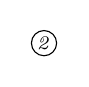
\begin{tikzpicture}\draw (0,0) circle (0.16cm) node {\textit{\scriptsize 2}};\end{tikzpicture}}%\! 
 C{\scriptstyle \textit{2}}B,\smallfrown {\scriptstyle \textit{3}}B{\scriptstyle \textit{2}}B}%
{\raisebox{-0.6ex}{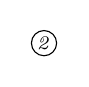
\begin{tikzpicture}\draw (0,0) circle (0.16cm) node {\textit{\scriptsize 2}};\end{tikzpicture}}%\! 
 C{\scriptstyle \textit{2}}A,\smallfrown {\scriptstyle \textit{3}}A{\scriptstyle \textit{2}}A}$.\rule[0mm]{0pt}{18pt} %
\pend
%
\pstart
Notandum est ubi post concursum\protect\index{Sachverzeichnis}{concursus} 
\rule[0cm]{0mm}{10pt}incipit discedendi iterum conatus,\protect\index{Sachverzeichnis}{conatus iterum discedendi} mutatis celeritatibus etiam centrum potentiae\protect\index{Sachverzeichnis}{centrum potentiae} mutari quod non amplius voco \textit{{\scriptsize2}C}, sed 
%
\raisebox{-0.6ex}{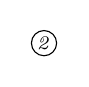
\begin{tikzpicture}\draw (0,0) circle (0.16cm) node {\textit{\scriptsize 2}};\end{tikzpicture}}\!\textit{C}.
%
\pend
%
\pstart 
Si ${\scriptstyle \textit{2}}B{\scriptstyle \textit{3}}B\,\groesser {\scriptstyle \textit{1}}B{\scriptstyle \textit{2}}B$, etiam ${\scriptstyle \textit{1}}A{\scriptstyle \textit{2}}A\,\groesser {\scriptstyle \textit{2}}A{\scriptstyle \textit{3}}A$ et %
\edtext{contra quia}{\lemma{contra}\Bfootnote{\textit{(1)}~ergo \textit{(2)}~si \textit{(3)}~\textbar\ porro \textit{streicht~Hrsg.}\ \textbar\ %
 \textit{(4)}~quia~\textit{L}}} %
%
ponimus \textit{{\scriptsize3}A} esse ab illa parte, a qua est centrum potentiae\protect\index{Sachverzeichnis}{centrum potentiae} \textit{{\scriptsize3}C} et fuisse ab eadem in casu %
\edtext{occursus,\protect\index{Sachverzeichnis}{occursus} jam}{\lemma{occursus,}\Bfootnote{\textit{(1)}~hinc \textit{(2)}~jam~\textit{L}}} %
%
 ante, seu fuisse sinisterius quam \textit{{\scriptsize2}A}. Hinc sive (\textit{{\scriptsize3}A}) cadat intra \textit{{\scriptsize1}A} et \textit{{\scriptsize2}A}, quo casu minuta est celeritas per
%
%
\edtext{occursum,\protect\index{Sachverzeichnis}{occursus} sive \textit{{\scriptsize3}A} cadat extra, erit recta}{\lemma{occursum, sive}\Bfootnote{\textit{(1)}~cadat extra in \textit{{\scriptsize3}A} \textit{(2)}~\textit{{\scriptsize3}A} cadat extra, erit \textit{(a)}~sem \textit{(b)}~recta~\textit{L}}} %
%
 \textit{{\scriptsize1}A}\textit{{\scriptsize3}A}, differentia inter \textit{{\scriptsize1}A}\textit{{\scriptsize2}A}, et \textit{{\scriptsize2}A}\textit{{\scriptsize3}A}. Posito ergo \textit{{\scriptsize3}A} cadere intra \textit{{\scriptsize1}A} et \textit{{\scriptsize2}A}, %
\edtext{tunc \textit{{\scriptsize2}A}\textit{{\scriptsize3}A} erit}{\lemma{}\Bfootnote{tunc \textbar\ tunc \textit{streicht~Hrsg.} \textbar\ \textit{{\scriptsize2}A}\textit{{\scriptsize3}A} erit~\textit{L}}} %
%
 minor quam \textit{{\scriptsize1}A}\textit{{\scriptsize2}A}. Ergo et \textit{{\scriptsize1}B}\textit{{\scriptsize2}B} erit minor 
%
\edlabel{37_05_152r_5a}%
quam \textit{{\scriptsize2}B}\textit{{\scriptsize3}B}.%
\edtext{}{{\xxref{37_05_152r_5a}{37_05_152r_5b}}\lemma{quam \textit{{\scriptsize2}B}\textit{{\scriptsize3}B}.}\Bfootnote{\textit{(1)}~Ergo si corpora \textit{(a)}~sibi \textit{(b)}~\textit{A}, \textit{B} sibi occurrunt, \textit{(aa)}~erit locus \textit{(aaa)}~post res \textit{(bbb)}~corporis \textit{A}, cui contrait centrum \textit{(bb)}~et centrum potentiae contrait corpori \textit{A}, tunc erit \textit{(2)}~In~\textit{L}}} %
%
\pend
\newpage
%
\pstart 
In\edlabel{37_05_152r_5b} 
%
quam partem it centrum potentiae,\protect\index{Sachverzeichnis}{centrum potentiae} in eam partem post occursum\protect\index{Sachverzeichnis}{occursus} ire necesse est %
\edtext{corpus ad}{\lemma{corpus}\Bfootnote{\textit{(1)}~quod \textit{(2)}~ad~\textit{L}}} %
%
cujus partem centrum potentiae\protect\index{Sachverzeichnis}{centrum potentiae} tendit, v.g.\ 
%
\edtext{quia centrum potentiae\protect\index{Sachverzeichnis}{centrum potentiae} it}{\lemma{quia}\Bfootnote{centrum potentiae \textit{(1)}~tendit \textit{(2)}~ab or \textit{(3)}~it~\textit{L}}} %
%
ordine \textit{{\scriptsize1}C}.\textit{{\scriptsize2}C}.\textit{{\scriptsize3}C}, versus \textit{{\scriptsize3}A}, hinc post occursum\protect\index{Sachverzeichnis}{occursus} necesse est 
%
\edtext{et \textit{{\scriptsize2}A}}{\lemma{et}\Bfootnote{\textit{(1)}~\textit{{\scriptsize3}A} tende \textit{(2)}~\textit{{\scriptsize2}A}~\textit{L}}} %
%
tendere versus \textit{{\scriptsize3}A}. Quaeritur jam in quam partem tendat corpus \textit{B}; si corpus \textit{A} post occursum\protect\index{Sachverzeichnis}{occursus} tendit celerius quam %
\edtext{prius, necesse est}{\lemma{prius,}\Bfootnote{\textit{(1)}~tendat, \textit{(2)}~necesse est~\textit{L}}} %
%
 ut corpus \textit{B} moveatur tardius, tantum quaeritur in quam %
\edtext{partem. Necesse}{\lemma{partem.}\Bfootnote{\textit{(1)}~Erit autem necessario eo casu \textit{(2)}~Necesse~\textit{L}}} %
%
est corpus cujus motus in contrariam partem augetur minus habere potentiae\protect\index{Sachverzeichnis}{potentia} quam id cujus %
\edtext{motus continuatur,}{\lemma{motus}\Bfootnote{\textit{(1)}~in contrariam \textit{(2)}~continuatur,~\textit{L}}} %
%
vel cujus motus in contrariam quidem sed minor est quam ante. Ergo 
%
\begin{tabular}[t]{lc}si&\textit{{\scriptsize2}A}${\scriptstyle \textit{3}}A\,\groesser $\textit{{\scriptsize1}A}\textit{{\scriptsize2}A},\\ 
seu&\textit{{\scriptsize1}B}${\scriptstyle \textit{2}}B\,\groesser $\textit{{\scriptsize2}B}\textit{{\scriptsize3}B}\end{tabular}
%
fuit \textit{{\scriptsize1}C}${\scriptstyle \textit{1}}B\,\groesser $\textit{{\scriptsize1}C}\textit{{\scriptsize1}A}. %
\pend
%
\pstart
Sit casus quo corpus magnum\protect\index{Sachverzeichnis}{corpus magnum} motum ingruit in parvum quiescens.\protect\index{Sachverzeichnis}{corpus parvum quiescens} 
%
\lbrack\textit{Text bricht ab.}\rbrack
%
\pend 
\count\Bfootins=1200%
\count\Afootins=1200%
\count\Cfootins=1200